
\documentclass{article}

% ----------------------- PAQUETES ---------------------- %
% Set the font (output) encodings
\usepackage[T1]{fontenc}					% encoding de la fuente
\usepackage[spanish]{babel}				% paquete para los acentos en español
\usepackage{graphicx}							% paquete para poder usar graficos
\usepackage{float}								% paquete para poder usar \begin {figure}[H]
\usepackage{xurl}					% https://stackoverflow.com/questions/4146606/wrap-url-ignores-margin-in-bibtex-using-pdflatex
\usepackage{hyperref}							% paquete para hacer hyperreferencias a links
\usepackage{fancyhdr}							% paquete para poner cosas en footer y header
\usepackage{wrapfig}							% paquete para hacer wrapfigure
\usepackage{titling}							% paquete para modificar el espaciado de los titulos
\usepackage{titlesec}							% paquete para modificar como se ven los titulos
\usepackage{todonotes}						% paquete para hacer todos
\usepackage{subfiles}							% paquete para hacer subfiles


% ------------------------------------------------------- %

% ---------------------- CONFIGURACION ------------------ %

\graphicspath{{images/}}
% ----------------- Configuracion de hyperref ----------- %
\hypersetup{								
	colorlinks=true,
	linkcolor=black,			%modo claro
	%linkcolor=white,		%modo oscuro
	filecolor=brown,		
	urlcolor=blue,
	pdftitle={Modelo de capacitación para uso de transporte público},
	}
% ------------------------------------------------------- %


%---------- headers y footers con fancyhdr ----------- %
\pagestyle{fancy}
	\setlength{\headheight}{12.17pt}
	%limpio el estilo
	\fancyhf{}
	
	%header
	\renewcommand{\headrulewidth}{1pt} %La linea horizontal
	\lhead{Librepass}
	\chead{}
	\rhead{Krapp Ramiro}

	%footer
	\renewcommand{\footrulewidth}{1pt} %La linea horizontal
	\lfoot{}
	\cfoot{}
	\rfoot{Pagina \thepage}
% ------------------------------------------------------- %


%-------------- Formatos de los titulos --------------%
\newcommand{\sectionbreak}{\clearpage}
\titleformat{\section}
	{\bfseries \huge \centering}
	{}
	{0em}
	{}[\titlerule]

\titleformat{\subsection}
	{\bfseries \Large}
	{}
	{0em}
	{}

\titleformat{\subsubsection}
	{\bfseries}
	{}
	{0em}
	{}[\hrule]


\titlespacing{\section} %me permite controlar el espaciado de la seccion que le indico
	{0em}
	{0em}
	{1.5em}

\titlespacing{\subsection}
{0em} %sangria
{3em} %separacion con lo que hay arriba
{0.5em} %separacion con lo que hay abajo
%----------------------------------------------------- %

% ----------------- FIN DE CONFIGURACION ------------- %

\begin{document}

\begin{titlepage}
	\begin{center}
		\vspace{1cm}

		{\Huge
			\textbf{Librepass}}

		\vspace{0.3cm}
		{\LARGE
			Informe técnico}

		\vspace{0.5cm}
		{\Large
			Un trabajo presentado para la materia de \\
			Emprendimiento Local y Desarrollo Productivo}

		\vspace{1cm}

		\begin{figure}[H]
			\centering
			
\includegraphics[width=0.7\textwidth]{../../informe/images/logo.png}
		\end{figure}

		\vfill

		{\Large
			\textbf{Krapp Ramiro} \\
			\vspace{0.5cm}
			Instituto tecnológico San Bonifacio\\
			Departamento de electrónica\\
			\today
		}

		\vspace{0.5cm}
		{\large Hecho en {\LaTeX}}

	\end{center}
\end{titlepage}

\section{Introducción}
%- Descripcion del producto
%- Resultados de las encuestas (como los graficos de tarta)
%- Conclusiones de las encuestas
%- Video corto de la entrevista
%
%Esto se entrega el 27

Librepass es un sistema de seguridad FOSS (Free and Open Source) implementado en
base a un sistema de lectores RFID, y con implementación en la nube.

Este está pensado para ser instalado en las puertas de las empresas en
las que se desea implementar una seguridad extra, y evitar la entrada de personas
no deseadas a ciertas habitaciones, o en todo caso, a la planta entera.

Esta diseñado para ser sencillo de usar e implementar, y presenta un sistema
sencillo de niveles de autorización que permite agregar complejidad al sistema
de forma que se vea necesaria.

Para su instalación, se provee un set de lectores y tarjetas con cantidad a elección.

\subsection{Ventajas del producto}
El producto presenta múltiples ventajas, en las cuales se incluyen:
\begin{itemize}
	\item Sencillez a la hora de instalarlo.
	\item Sencillez a la hora de configurarlo.
	\item Sencillez a la hora de usarlo.
	\item Precio económico.
	\item Escalabilidad
	\item Cumplimiento de las 4 libertades esenciales del software libre:
	      \begin{enumerate}
		      \item La libertad de correr el programa como se desee, para cualquier propósito
		      \item La libertad de estudiar cómo el programa funciona, y cambiarlo para que
		            haga lo que el usuario desee.
		            El acceso al código fuente es una precoindición para lograr esto
		      \item La libertad para redistribuir copias así puedes ayudar a los demás.
		      \item La liberta de distribuir copias de tus versiones modificadas a otros.
		            Haciendo esto, le puedes brindar a toda la comunidad una chance de beneficiarse
		            de tus modificaciones.
		            El acceso al código fuente es una precoindición para lograr esto
	      \end{enumerate}
\end{itemize}

\begin{figure}[H]
	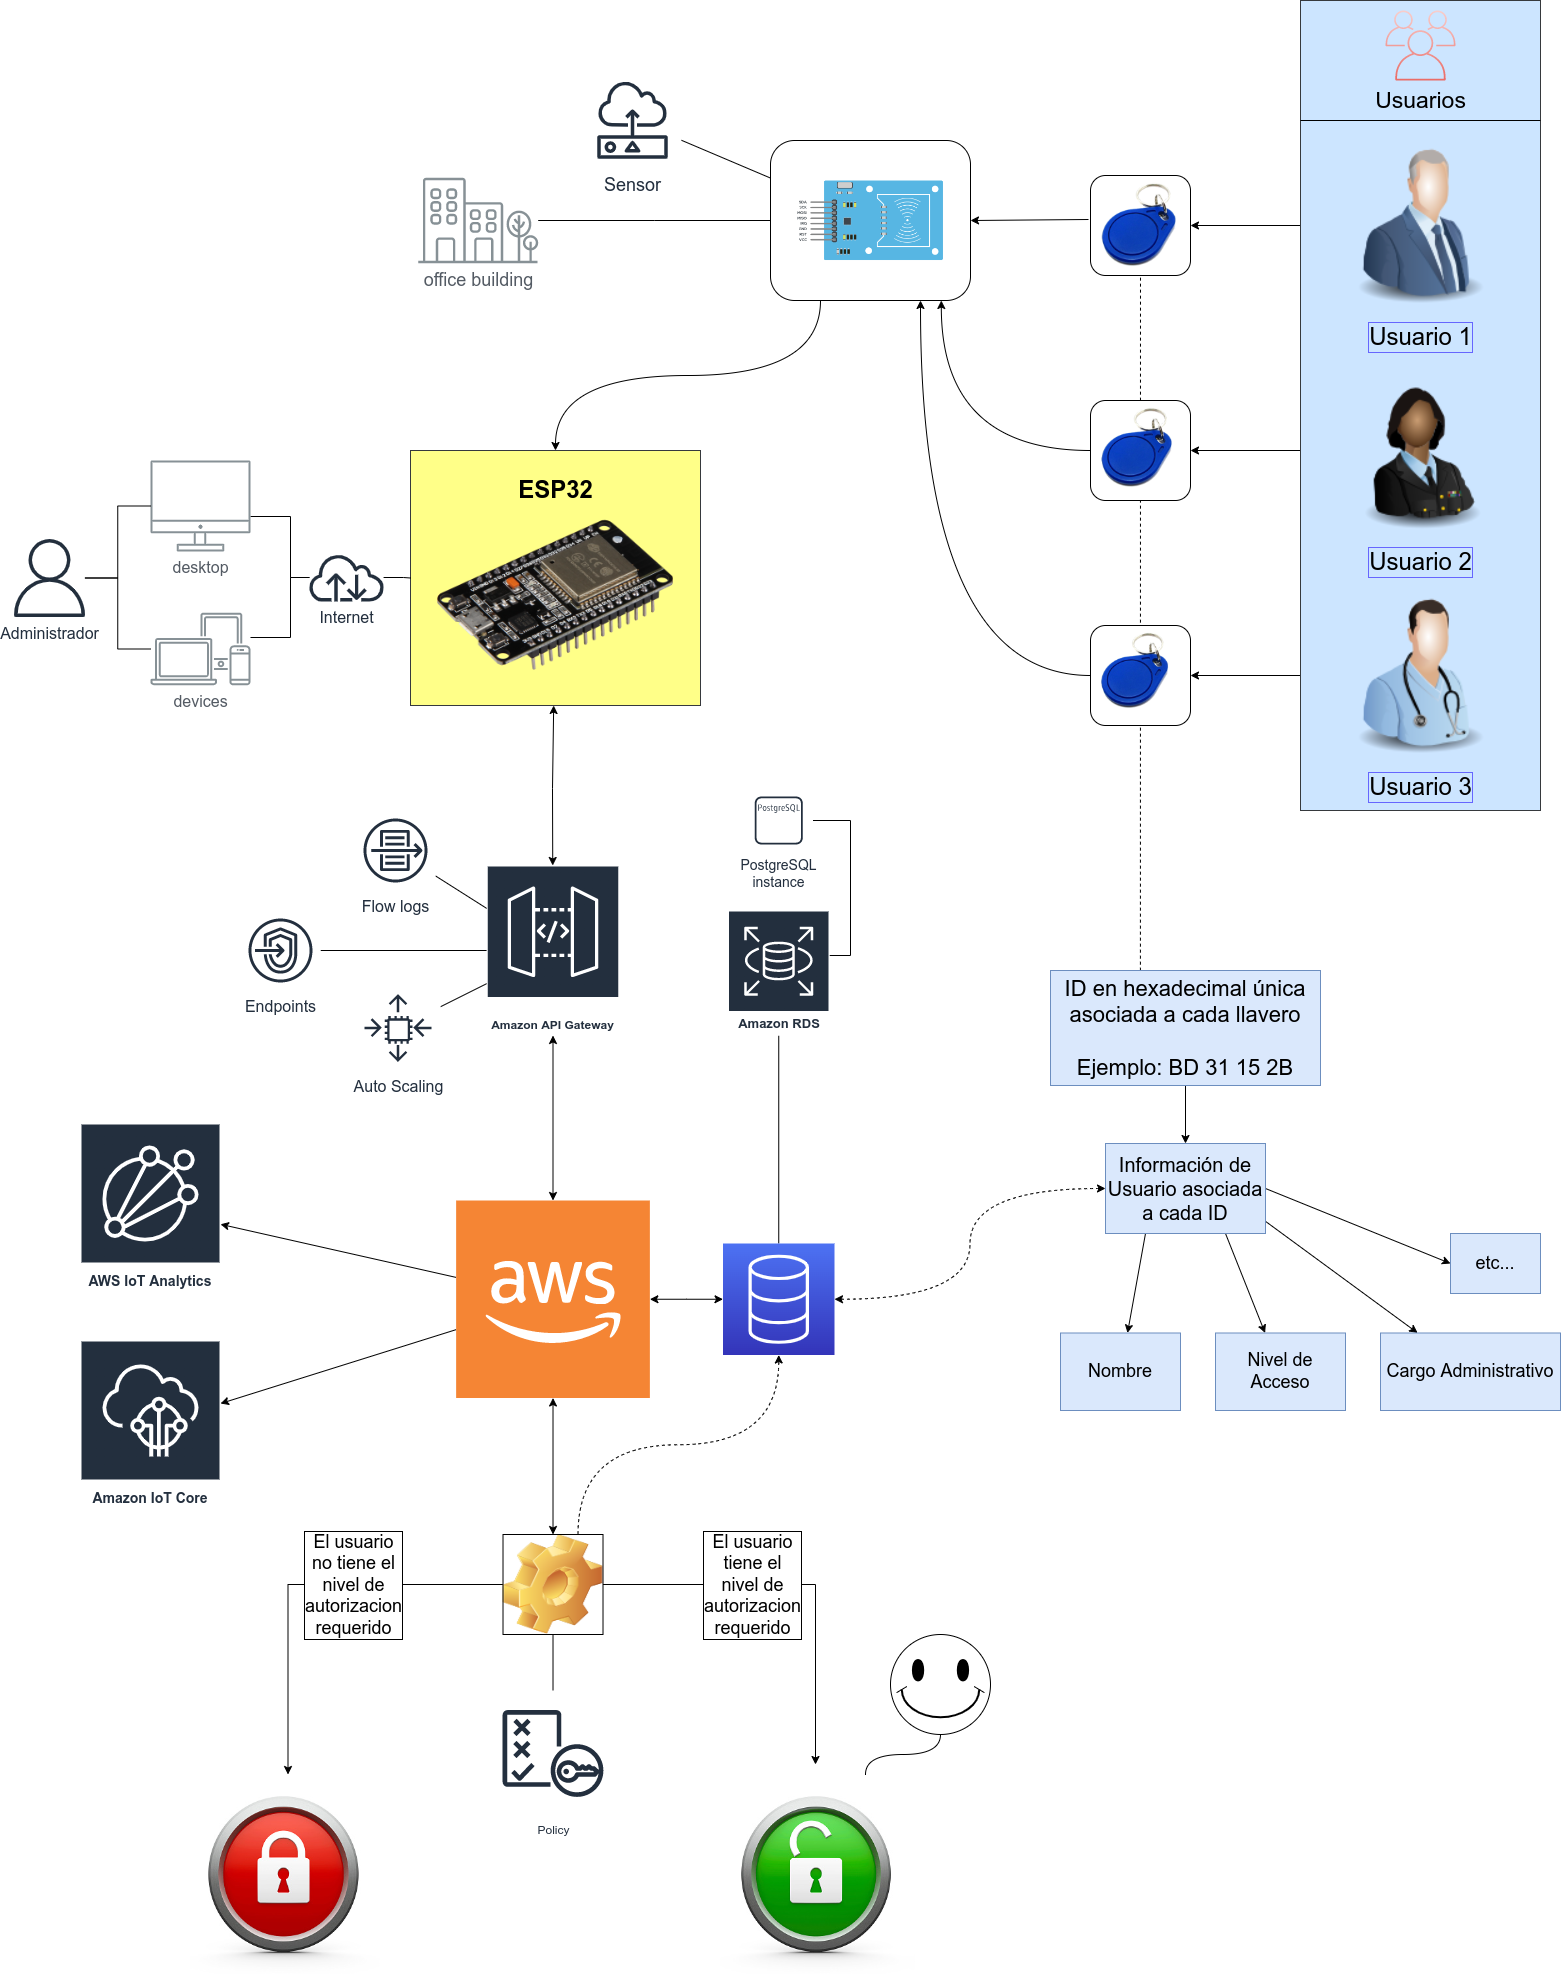
\includegraphics[width=\textwidth]{../../informe/images/diagrama.drawio.png}
	\centering
	\caption{Un diagrama del modelo}
\end{figure}

\clearpage

\subsection{Aplicaciones alternativas de la tecnología}
Esta tecnología se puede aplicar y modificar para los siguientes usos:
\begin{itemize}
	\item Un sistema de indentificación de identidad de animales domésticos.
	\item Un sistema de registro de ingreso y egreso
\end{itemize}

\section{Resultados de las encuestas}
De las encuestas se pueden notar multiples cosas:
\begin{enumerate}
	\item La tendencia de edad está entre los 18 y 60 años. Esto quiere decir que no hay un grupo etario muy marcado
	\item Es notable como la mayoría de los entrevistados tiene cierto conocimiento de los programas de código abierto.
	      Esto se cree que puede ser porque los entrevistados buscaron en internet que eran los programas de codigo abierto,
	      y al hacerlo se enteraron que usaban multiples programas del estilo, como VLC, Firefox, Blender, OBS Studio, qBitTorrent,
	      Audacity, etc...
	\item Se le suele dar una importancia notable a la seguridad en las empresas. Esto quiere decir que nuestro producto es relevante.
	      Tambien se ve una gran sensacion de necesidad del aumento de la seguirdad.
	\item Es claro como las personas buscan que los sistemas sean sencillos de usar y tambien se busca
	      que de muchas opciones a la hora de configurar, y, en contraste, se dio que hay una buena cantidad de personas que piden que sea minimalista.
	      De esto se puede concluir de que se pueden incluir dos posibles opciones en la configuración:
	      Una que sea un modo sencillo, y otro avanzado, como se hace en las BIOS de ASUS con su EZ Mode
\end{enumerate}

\begin{figure}[H]
	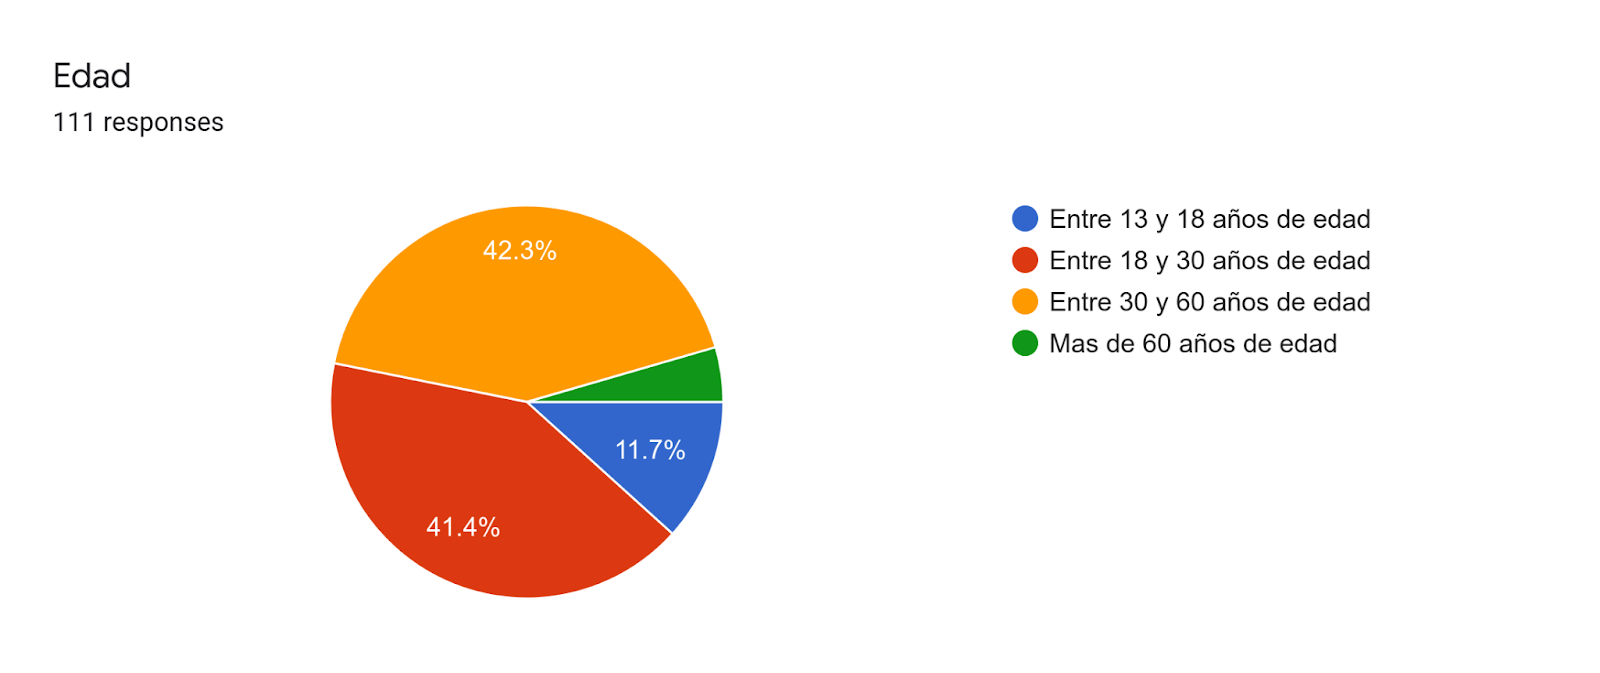
\includegraphics[width=\textwidth]{1.png}
	\centering
	\caption{Se puede notar como la tendencia de edad está entre los 18 y 60 años}
\end{figure}
\begin{figure}[H]
	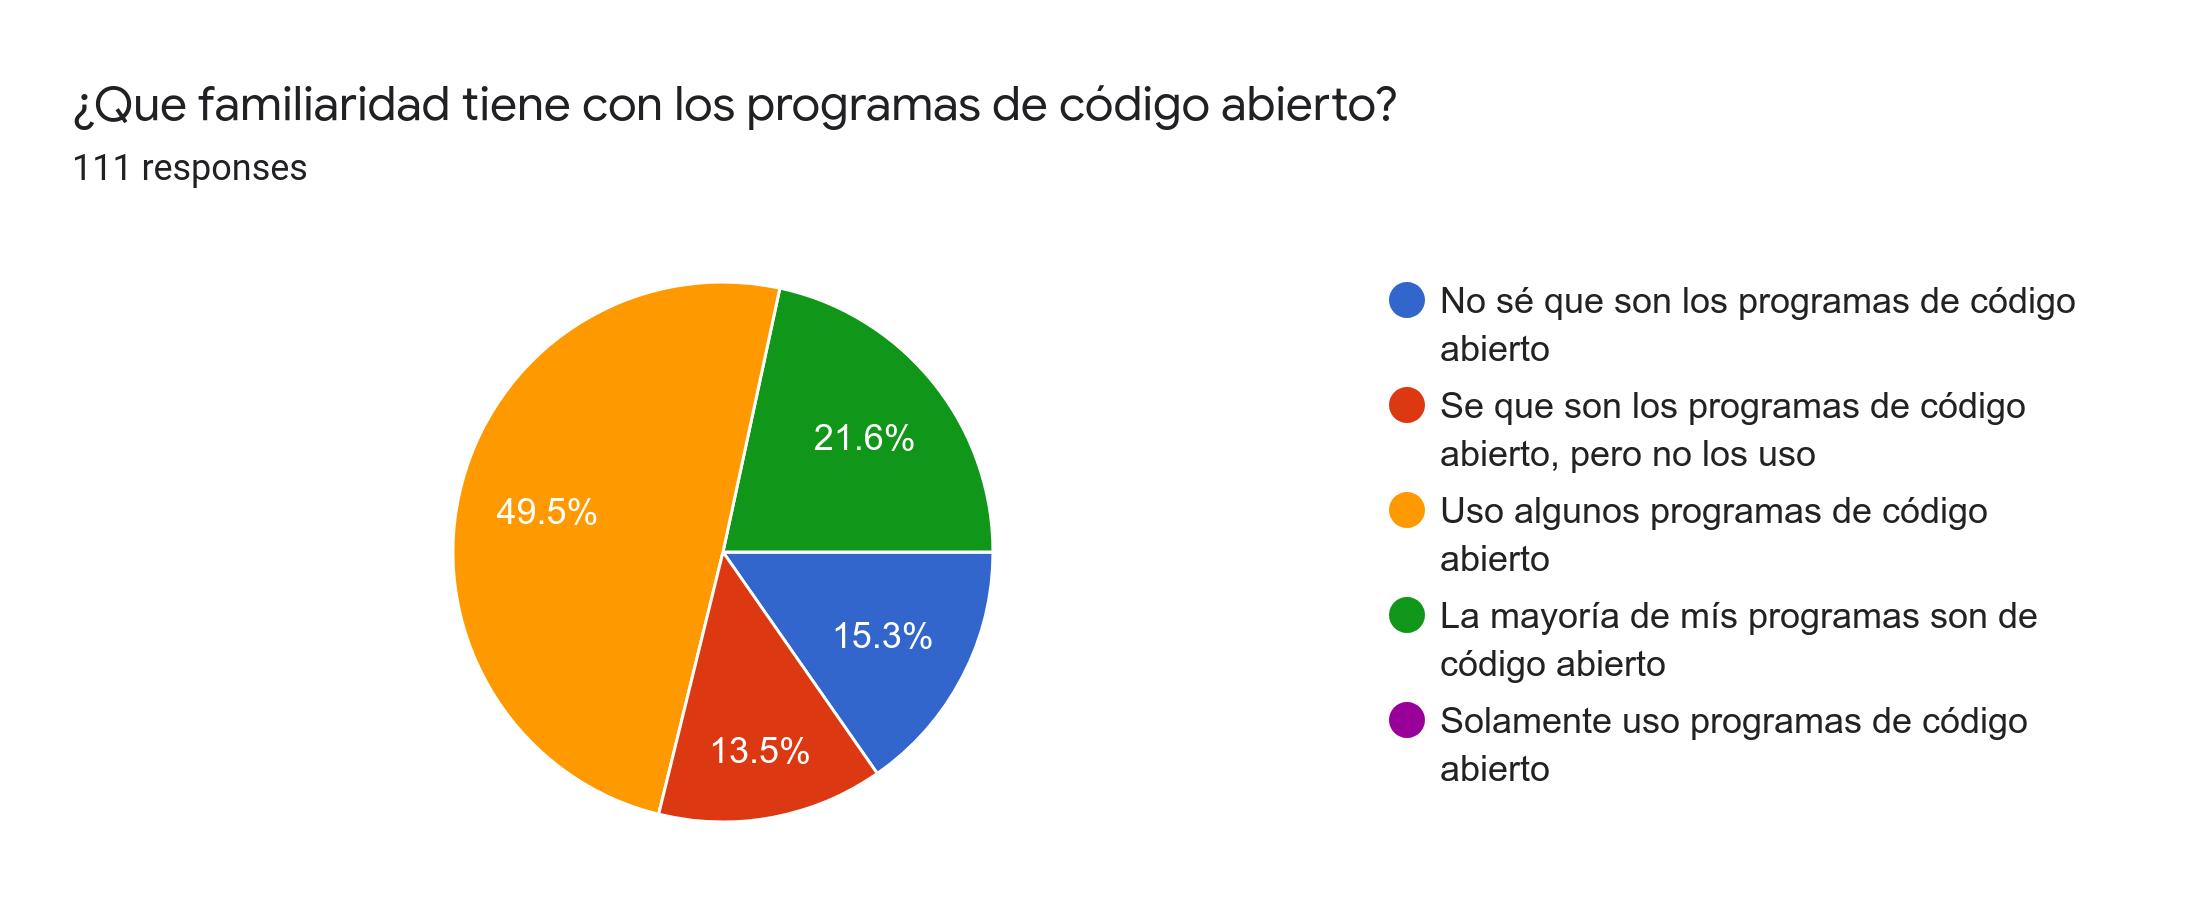
\includegraphics[width=\textwidth]{2.png}
	\centering
	\caption{Se puede notar cómo la mayoría de las personas usa algunos programas de código abierto}
\end{figure}
\begin{figure}[H]
	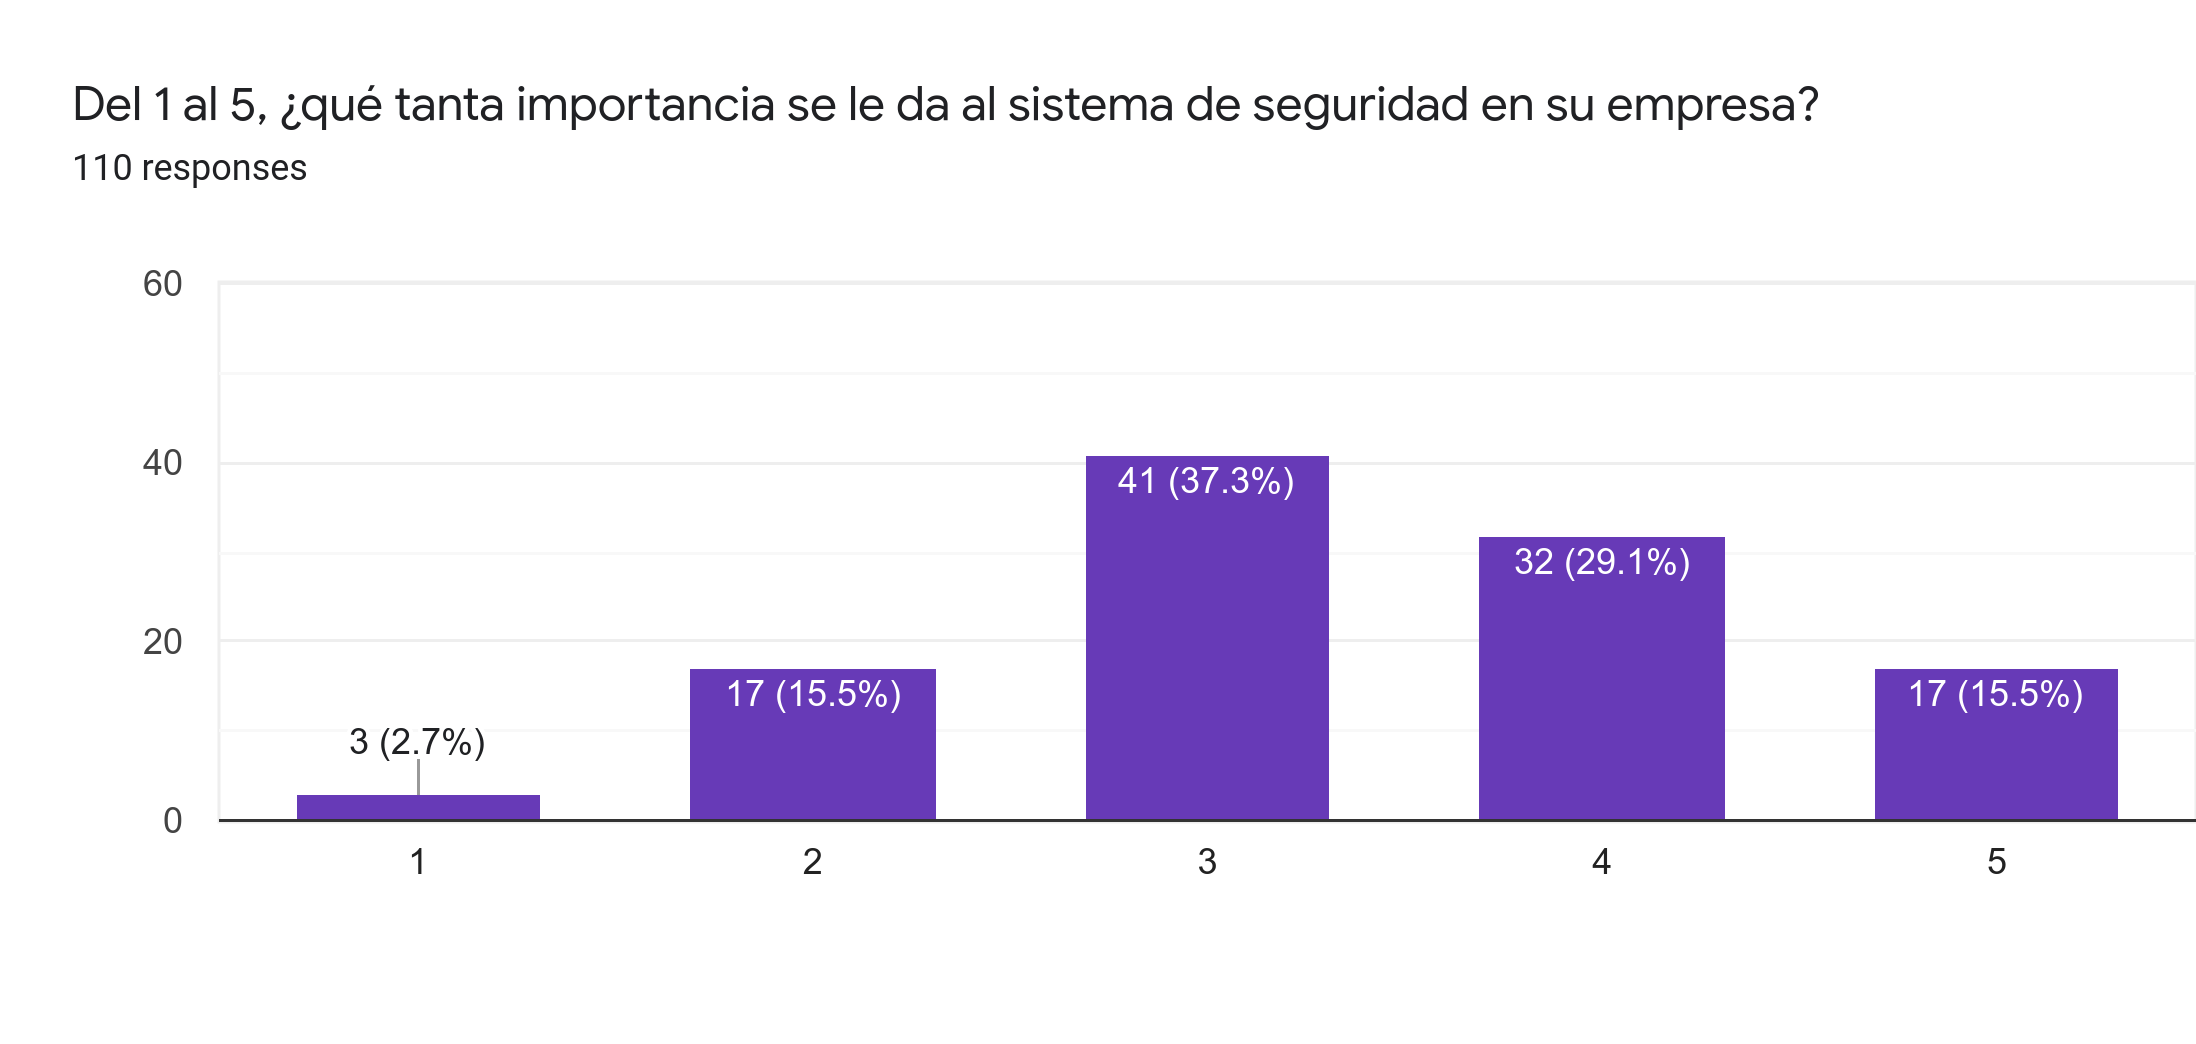
\includegraphics[width=\textwidth]{3.png}
	\centering
	\caption{Se puede notar como la importancia hacia la seguridad en las empresas es una campana de Gauss corrida a la derecha}
\end{figure}
\begin{figure}[H]
	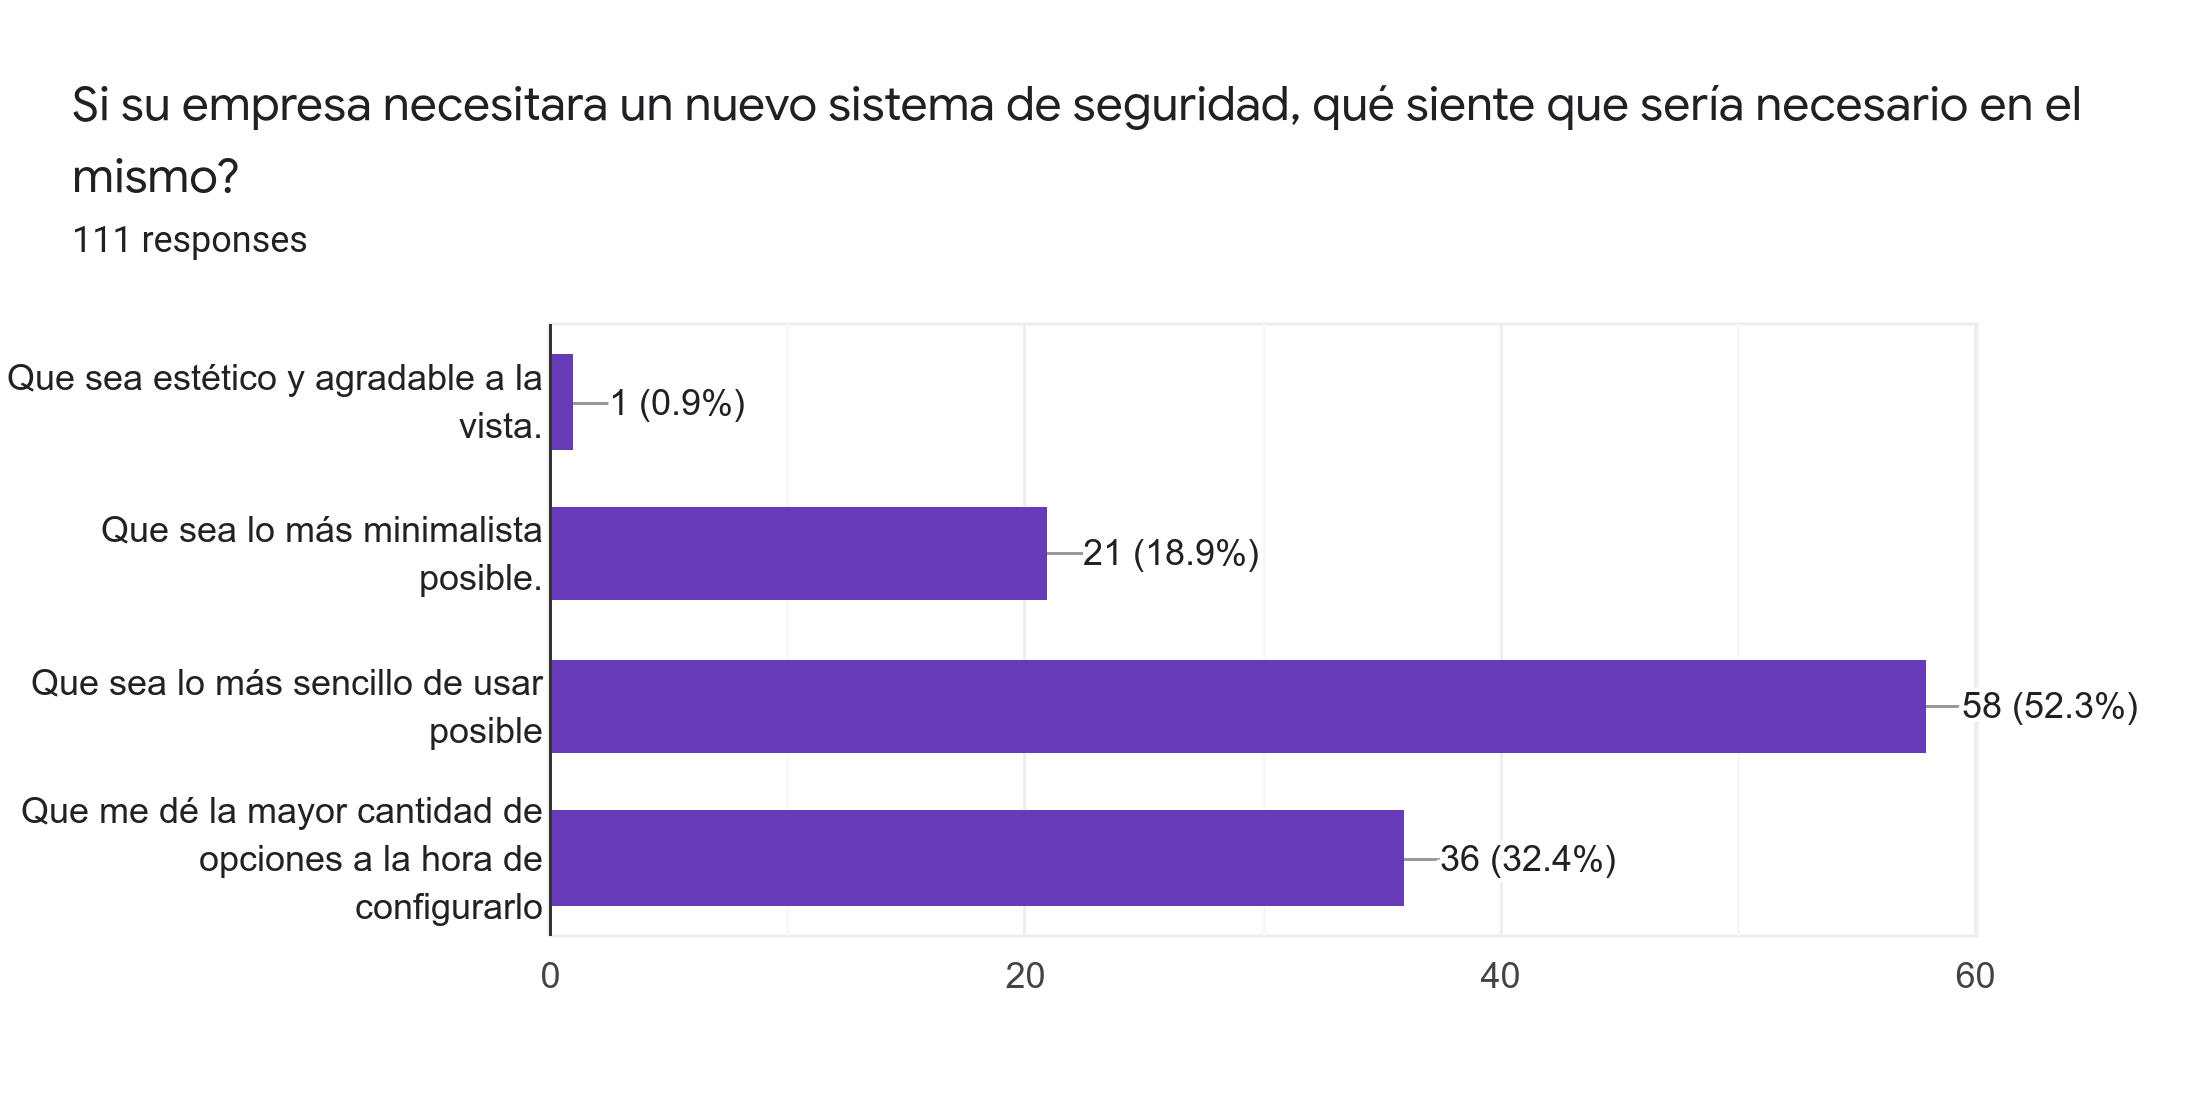
\includegraphics[width=\textwidth]{4.png}
	\centering
	\caption{Se puede notar como la mayoría de las personas buscan que sea lo más sencillo de usar}
\end{figure}
\begin{figure}[H]
	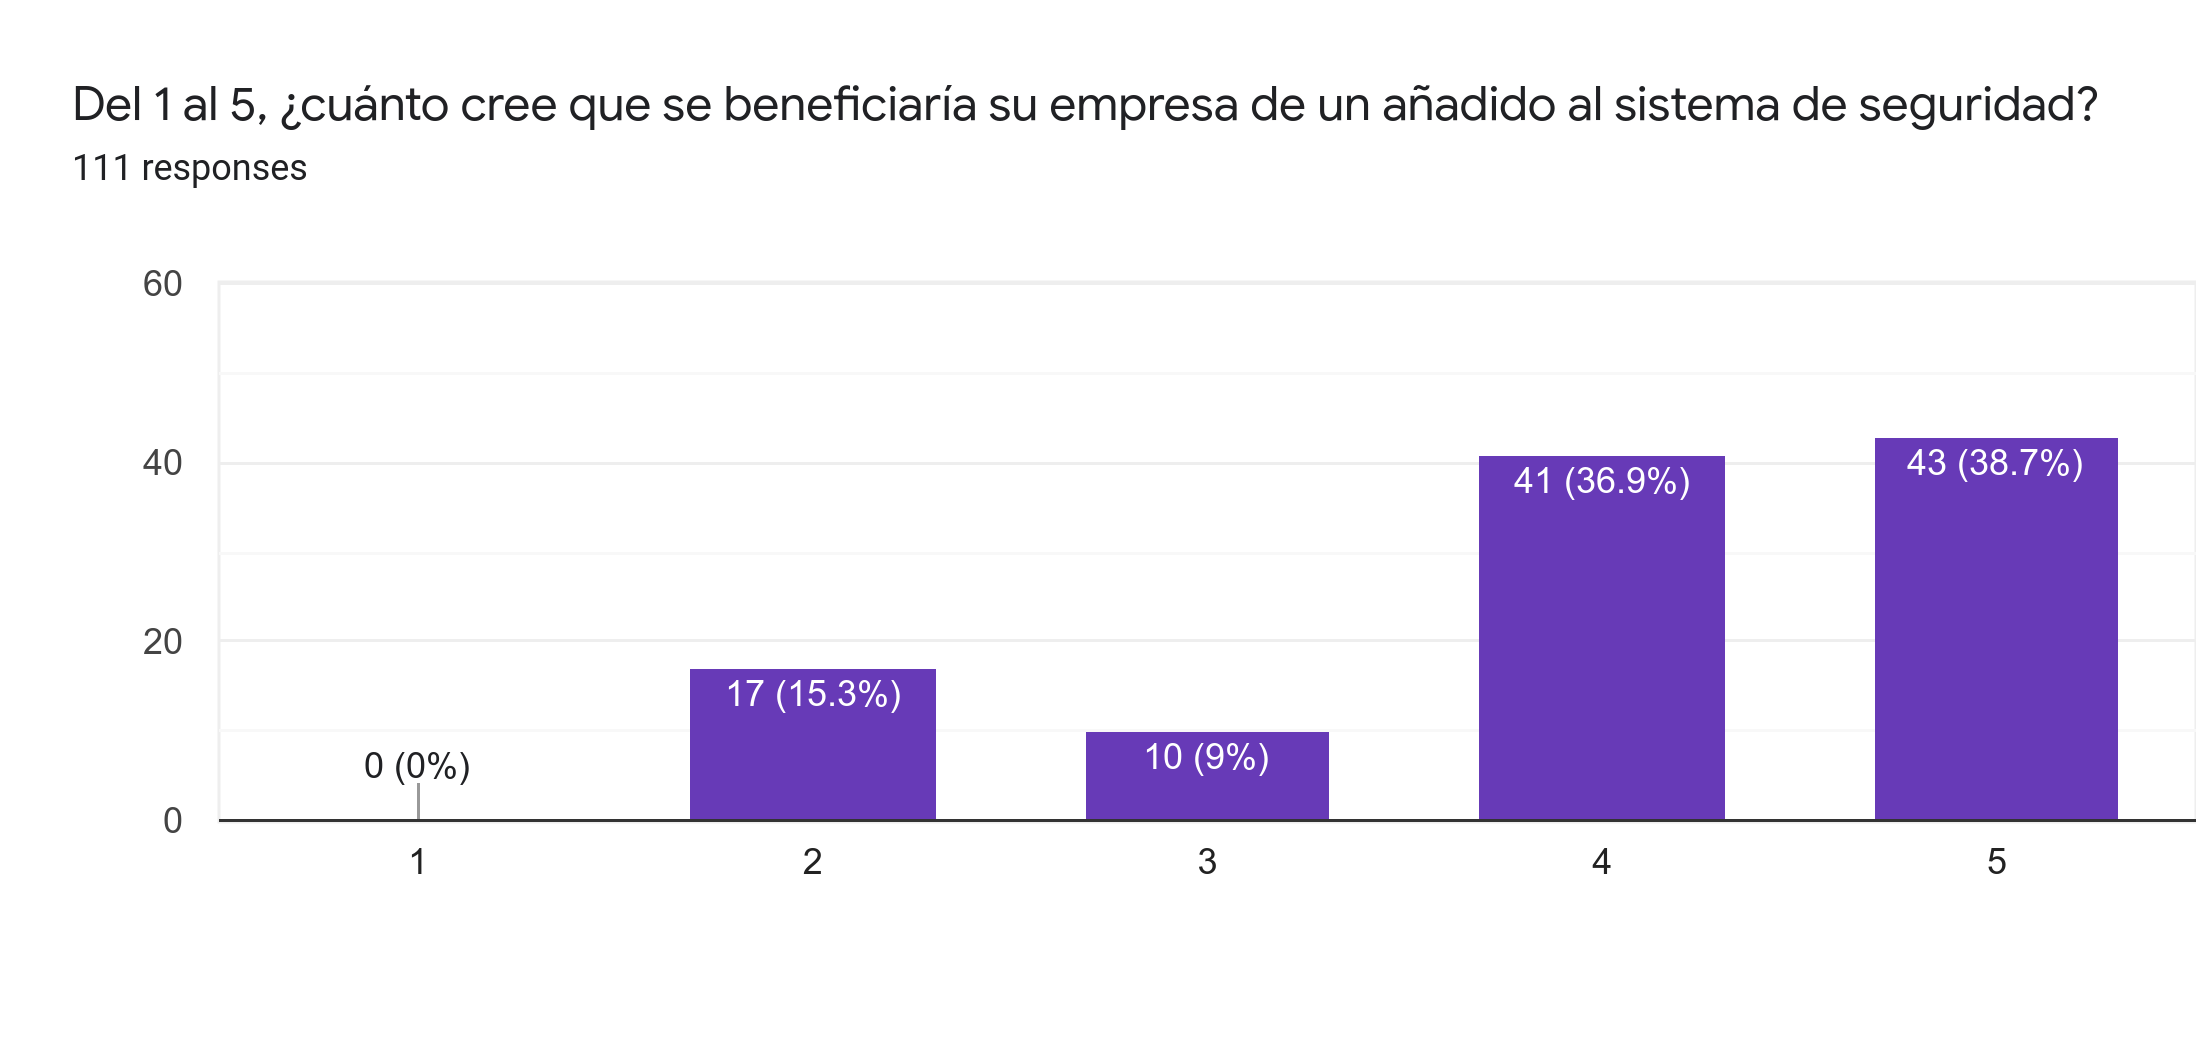
\includegraphics[width=\textwidth]{5.png}
	\centering
	\caption{Es evidente cómo las personas creen conveniente un añadido al sistema de seguridad de sus empresas}
\end{figure}

\section{Resultados de las entrevistas}
\subsection{Entrevistado Numero 1}
\subsubsection{Nombre}
Marcos

\subsubsection{Profesion}
NodeJs Developer

\subsubsection{Edad}
24 años

\subsubsection{Hace cuanto trabaja en el area de sistemas/programacion?}
Si cuento desde que doy cursos (mi primer trabajo formal), diria que desde fines del 2018, y mi primer trabajo como programador fue mayo del 2019

\subsubsection{Tiene estudios universitarios?}
Analista Universitario en Sistemas de Informacion

\subsubsection{¿Tiene experiencia con los sistemas cloud? ¿Qué opina de ellos?}
Si, tengo bastante experiencia. Hace un tiempo que vengo trabajando con soporte cloud, en mi experiencia laboral use Firebase y AWS, y en el ámbito personal use Heroku. En si me parece que el termino se hace mucha propaganda porque es algo nuevo, pero en realidad el concepto es algo que ya existía, el alquiler de servidores.

El cloud en realidad es la computadora de otra persona, lo que no había es a nivel estratosférico que hay hoy en día de las grandes empresas. Lo que tampoco había era el sistema de micro servicios de hay hoy en día.

Lo que tiene de ventajoso el cloud es que la otra alternativa, hacer tu propio servidor es algo caro, y nunca le vas a poder ganar a google o a amazon en su capacidad de "hosting", entonces es mucho más barato. Ademas permite hacer el sistema más expansible.

En mi empresa el cloud nos permitió que en casos como en la noche, se pueden des escalar los servicios, y permite tener un uso más económico del servicio, por lo cual es más flexible.

Hoy en día cualquier programador necesita saber lo básico de cloud.

\subsubsection{¿Considera que los sistemas cloud son seguros?}
Eso depende. Son tan seguros como vos los configures, obviamente se pueden hacer cosas muy seguras, dependiendo que tanto pagues también. Los sistemas muy seguros son caros.

Hay una desventaja también en los sistemas cloud, que es la situación "que pasa si google/amazon se funden", lo cual, como programadores, creemos que es muy poco probable.

Además, los datos de cloud están en el extranjero, lo cual legalmente los pone en una situación distinta. Esto ya pasó con MegaUpload. Por ejemplo, el banco central no les permite a los otros bancos tener datos de los clientes y transacciones en sistemas cloud, por una cuestión legal, para evitar eso.
O sea, nosotros en los bancos usamos cloud, pero los datos sensibles están en data-centers acá en argentina. Lo que ponemos en cloud son las aplicaciones, los micro servicios, el backend, algunas bases de datos de utilidad (logs)

En el tema de seguridad, usamos Auth0, la cual es uno de los unicornios argentinos, y nos provee a nosotros los Tokens para los servicios.

\subsubsection{¿Tiene experiencia con el mundo del IoT?}
No demasiada.

\subsubsection{¿Considera que el IoT es seguro?}
Es tan seguro como lo configures. El dispositivo IoT debería ser solamente un intermediario de los datos, y no para almacenarlos.

\subsubsection{¿Cuando piensa en sistemas de seguridad, que ejemplos se le vienen a la cabeza?}
Sistemas de autenticación y/o autorización de acceso de datos y servicios.

\subsubsection{¿Qué considera que tiene que tener un sistema de seguridad para ser bueno?}
Si pensamos en seguridad fisica, se estila usar politicas de seguridad, como tarjetas de acceso, camaras de seguridad, reconocimiento biométrico.

En seguridad de sistemas, se estila usar tokens de autenticacion y 2FA. Lo que tiene de bueno el 2FA es que las contraseñas suelen ser inseguras, pero el 2FA soluciona eso añadiendo una capa extra de seguridad.

\subsubsection{Alguna otra cosa que quieras comentar?}
Para tu proyecto, te convendria crear una REST API en heroku e ir consultando a un endpoint, como para empezar.

\subsubsection{Conclusiones de la entrevista}
Convendria hacer el desarrollo inicial en Heroku, para luego hacer el deploy de produccion a AWS. Es buena la opción de usar cloud,
ya que permite usar mejor el sistema monolítico, y es más barato. No es conveniente almacenar datos sensibles en cloud (como datos bancarios),
y el servicio cloud debería estar bien configurado.
Es conveniente crear una REST API.

\clearpage

\subsection{Entrevistado Numero 2}
\subsubsection{Edad}
22

\subsubsection{Hace cuanto trabaja en el area de sistemas/programacion?}
Desde el 2015

\subsubsection{Tiene estudios universitarios?}
No, pero hice la secundaria técnica en Informática y Redes

\subsubsection{¿Tiene experiencia con los sistemas cloud? ¿Qué opina de ellos?}
Si, tengo 2 años de experiencia manejando tecnologías cloud, y en el tiempo recorrido he notado la necesidad de implementación de este tipo de tecnologías para agilizar la arquitectura sobre el desarrollo de las distintas aplicaciones y el tiempo de desarrollo de las mismas.

\subsubsection{¿Considera que los sistemas cloud son seguros?}
Depende de quien los maneje, y el tipo de configuración. Eso depende de como configures el servicio de S3 de Amazon, ese lo podes configurar que sea publico, y si lo agarra alguien que no tenga mucha experiencia y lectura en el tema puede ser bastante inseguro, por eso hay que estar bien informado, el que hace la arquitectura tiene que ser alguien con experiencia.

\subsubsection{¿Tiene experiencia con el mundo del IoT?}
Si, confio plenamente en la automatización de las cosas del hogar, cualquier cosa que me haga hacer menos, bienvenido sea. Como buen programador, puedo pasar 2 horas automatizando tareas de 10 minutos.

Por ejemplo, en casa tengo todas las luces las tengo conectadas a un switch wifi con el asistente de google, y tengo configurado para que se pueda cambiar el color, la intensidad, horarios de encendido y apagado, etc...

\subsubsection{¿Considera que el IoT es seguro?}
No, en lo absoluto, en lo más mínimo. Por algo los especialistas en seguridad informática no tienen nada automatizado en la casa

\subsubsection{¿Cuando piensa en sistemas de seguridad, que ejemplos se le vienen a la cabeza?}
Alarmas, cámaras de seguridad, sensores de movimiento, VPN's, VPC (conecta dos subnets que no estan conectadas al internet exterior, esto se suele hacer en cloud) y sistemas de entrada usando RFID.

\subsubsection{¿Qué considera que tiene que tener un sistema de seguridad para ser bueno?}
Multiples factores de autenticación y backups de respaldo en caso de perdida de datos y/o energía.

\subsubsection{Alguna otra cosa que quieras comentar?}
Para la base de datos, podrias usar mongoDB o PostreSQL. En AWS podes usar el servicio EC2

\subsubsection{Conclusiones de la Entrevista}
Hoy en dia son cada vez más requeridos los sistemas cloud. Estos son seguros dependiendo de que tan bien se configuren, y por
lo general la arquitectura la hace alguien con experiencia. Un buen sistema de seguridad debería tener multiples factores de autenticación 
y backups de respaldo en caso de perdida de datos y/o energía. Para la base de datos, podria usar mongoDB o PostreSQL.
En AWS puedo usar el servicio EC2

\end{document}